\documentclass[transmag]{IEEEtran}
\usepackage{latexsym}
\usepackage{graphicx}
\usepackage{bbm}
\usepackage{amsfonts,amssymb,amsmath}
\usepackage{hyperref}
\def\BibTeX{{\rm B\kern-.05em{\sc i\kern-.025em b}\kern-.08em T\kern-.1667em\lower.7ex\hbox{E}\kern-.125emX}}
\markboth{$>$ EE369 Course Project $<$}
{$>$ EE369 Course Project REPORT $<$}
\begin{document}

\title{Implementation of Fully Convolutional Network for Semantic Segmentation in Pixel-level}

\author{Haotian Xue 518021910506\\
xavihart@sjtu.edu.cn   \\ https://github.com/xavihart}


\IEEEtitleabstractindextext{\begin{abstract}
  This is the report for EE369 Course Project. This project mainly focuses on the integrated Implementation of Fully Convolutional
  Network(FCN) proposed by Jonathan Long in CVPR2015. All the source codes can be referred to in my github:
  \textit{https://github.com/xavihart/MLProj-FCN-pytorch}. I built up the whole structure by pytorch and train it 
  on NVIDIA GTX 1080Ti. It took me about 5 hours to go through all the 300 epochs. In the report, I will briefly introudce the
  structure of FCN and illustrate the implementation of FCN in detail. At the end of this report, some thoughts are given about 
  this practice. It should be noted that the FCN in this report is FCN8s in the paper above.






\end{abstract}

}

\maketitle

\section{INTRODUCTION OF FCN}
\subsection{Differences from the traditional CNNs}
  Fully Convolutional Network(FCN)\cite{1} is a structure proposed by Jonathan Long et al. in CVPR2015. The significant diference between FCN and 
  normal CNN is that FCN is purely constructed of convolutional layers(including activation and pooling). We all know that the traditional CNNs used 
  for object classification tasks are made up of two main part: Conv layers for features extraction and FC layers for classification. The FC layers 
  facilitates the classification work though, it restrict and whole network: the input should always be the same size. For example $224 \times 224$ for 
  vgg16 and $28 \times 28$ for LeNet. FCN solves this question to a great extent by replacing the FC layer with Conv layer. This alternation actually made 
  no difference to the network structure, however it no longer has a restriction on the size of input. 
  
  For example, the last Conv layer ouputs a feature map sized of $512 \times 7 \times 7$, and you can use a filter sized of $4096 \times 512 \times 1 \times 1$
  instead of directly connect the $512 \times 7 \times 7$ value to a $1 \times 4096$ vector.

  In this way, if your input if $ b \times c \times h \times w$, after the downsampling process the output may be $b \times c^{'} \times \frac{h}{l} \times \frac{w}{l}$ 
  (in the traditional CNNS the last two dimension of the ouput can be seemed as 1). So the output is actually a bounch of feature map, 
  setting the number of bunches and you can train FCN to complete Semantic Segmentation work.

\subsection{Using FCN for semantic segmentation}
  Semantic segmentation is a kind of tasks which require the model to divie a image into semantic parts in pixel-level. This kind of tasks
  are always quite challenging becuase traditional CNNs cannot recognize a image in pixel level, the structure restrict it to cast the whole
  image into a category. FCN can do this job by upsampling the feature map ouput by the last Conv layer into the same size as the input image(
    channel numbers may be different.), the whole structure are shown in Fig. $1.^{[1]}$(This is the raw image from \cite{1}) To make the 
    outline information of the segmentation more clear, a jumping structure are made: it upsampled the feature map in the 4th and 3th layer of 
    vgg16 to join in the training process, which were proved to combine low features with high abstract features to polish the performence of 
    the whole structure. This model is specifically referred to as FCN8s.


\begin{figure}
\centerline{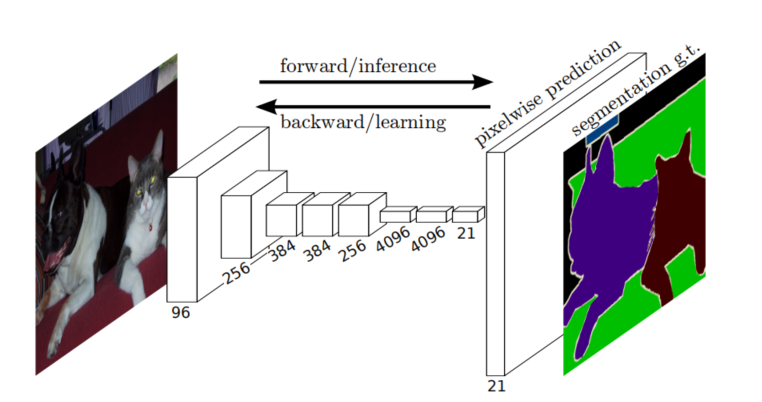
\includegraphics[scale=0.5]{model_structure.PNG}}
\caption{This is a visualized structure of FCN. It can make semantic segmentation for a image in pixel level.\label{fig1}}
\end{figure}


\begin{table}
  \centering
\caption{Key components and their detailed implementations}
\label{table}
\setlength{\tabcolsep}{3pt}
\begin{tabular}{|p{75pt}|p{125pt}|}
\hline
Key component & Implementation \\
\hline
Dataset    &        PASCAL-VOC2012             \\
Dataloader &   torch.utils.data.DataLoader        \\
Feature extract   &      VGG16               \\
upsampling   &       torch.nn.ConvTranspose2d               \\
Loss function   &        torch.nn.NLLLoss             \\
Optimizer   &           RMSprop          \\
Testing metrics  &      AP/mAP/mIoU               \\
Epoch number & 300 \\
Learning rate & first 20 epoch: $10^{-4}$ then $10^{-6}$ \\
 Devices            &      NVIDIA GTX 1080Ti $\times4$              \\

\hline

\hline
\end{tabular}
\label{tab1}
\end{table}





\section{KEY DESGINS OF THE IMPLEMENTATION}
The implementation are made up of three main parts: preparing datasets, building models and training/testing the models.
\subsection{Datasets prepration}
 The dataset used in the implementation is PASCAL-VOC2012(http://host.robots.ox.ac.uk/pascal
 /VOC/voc2012/index.html) segmentation task, there are
 totally 21 classes of objects in the dataset including 20 objects like dog, cat, bus... and 1 background. After unzipping the file downloaded from
 the website, I use voc-base.py to read the data and write a class inheritating torch.utils.data.DataLoader to restore the transformed image.
I use cv2.INTER-LINEAR and cv.INTER-NEAREST to resize the image and ground truth label respectively.Some example figrues can be referred to in 
Fig .2.
\begin{figure}
  \centerline{\includegraphics[scale=0.5]{vocexp.pdf}}
  \caption{Some example figures in VOC2012
  segmentation task and their segmentation ground truth.\label{fig2}}
  \end{figure}
\subsection{Building FCN8s model}
  The structure of FCN8s includes two parts, one of it is the VGG16 model\cite{2}, which are pretrained on 
  ImageNet\cite{3} and are utilized to extract features. Another important part is the upsampling layer, I use deconvolution as the
  upsampling method and build the whole structure on pytorch 1.2.0. Detailed message can be found in Table 1.
\subsection{Training and testing}
  The choose of loss function bothered me a lot in the beginning. By asking for other trainers help, I found that NLLLoss can be applied to 
  a multiclass segmentation like this, we define x as the input and y as the output. Normally, the dimension of x can be noted as $b * c * h * w$ and the dimension 
  of y can be noted as $b * h * w$, b refers to batch size, c is the number of categories and w * h is the spatial size of input image.The NLLLoss can be
  calculated as follows:

\begin{gather}
SX = Softmax(x, dim=1) \\
Mask(y, c)[i][j] = \mathbb{I}(y[i][j] == c)  \\
loss(x, y) = -\sum_{i=0}^{b-1} \sum_{j=0}^{c-1}{log(SX_{i,j}) * Mask(y, j)}
\end{gather}

The details about optimizer, learning rate... can be found in Table 1.
The testing metrics includes:AP(3), mAP(4) and mIoU(5), we assume $p_{ij}$ as the number of class i be predicted as class j.
respectively. s represents for the total number of pixels and c is the class number.
\begin{gather}
     AP  =  \frac{\sum_{i}p_{ii}} {s}              \\
     mAP = \frac{\sum_{i}{(p_{ii} / \sum_{j}p_{ij}})}{c}                     \\
     mIoU = \frac{\sum_{i}\frac{p_{ii}}{\sum_{j}p_{ij} + \sum_{j}p_{ji} - \sum_{i}p_{ii}    }}{c} 
\end{gather}


\section{EXPERIMENT RESULTS}


\subsection{Training process}
According to different kind of mistakes, I spent a lot of time training 








\begin{thebibliography}{00}
\bibitem{1} Long, Jonathan, Evan Shelhamer, and Trevor Darrell. "Fully convolutional networks for semantic segmentation." Proceedings of the IEEE conference on computer vision and pattern recognition. 2015.
\bibitem{2} Simonyan, Karen, and Andrew Zisserman. "Very deep convolutional networks for large-scale image recognition." arXiv preprint arXiv:1409.1556 (2014).
\bibitem{3} Deng, Jia, et al. "Imagenet: A large-scale hierarchical image database." 2009 IEEE conference on computer vision and pattern recognition. Ieee, 2009.
\end{thebibliography}
\end{document}
